\documentclass[11pt,a4paper]{article}

% These are extra packages that you might need for writing the equations:
\usepackage{amsmath}
\usepackage{amsfonts}
\usepackage{amssymb}
\usepackage{booktabs}
\usepackage{hyperref}
\usepackage{listings}
\usepackage{xcolor}

% You need the following package in order to include figures in your report:
\usepackage{graphicx}

% With this package you can set the size of the margins manually:
\usepackage[left=2cm,right=2cm,top=2cm,bottom=2cm]{geometry}


\begin{document}

% Enter the exercise number, your name and date here:
\noindent\parbox{\linewidth}{
 \parbox{.25\linewidth}{\large HPCSE, HW 5, Task 2}\hfill
 \parbox{.5\linewidth}{\begin{center} \large Beat Hubmann \end{center}}\hfill
 \parbox{.2\linewidth}{\begin{flushright} \large May 12, 2019 \end{flushright}}
}
\noindent\rule{\linewidth}{2pt}

\section{Task 1: Heat2D on CUDA}
To be submitted separately as optional bonus task before May 27, 2019.

\section{Task 2: Optimizing the N-body problem}
\subsection{Introduction}
After studying the supplied naive reference solution code and while doing some initial research,
I stumbled on the article~\cite{shuffle}. I then decided that it would be rewarding
to compare a complete rewrite of the code using warp shuffles with an implementation using
shared memory instead of doing the ablation study somewhat prescriptively suggested by the
benchmark table published on Piazza.\\
Thus, two implentations (warp-based, shared memory-based) of an improved force calculation kernel where written and compared
in terms of obtained performance. The more efficient one then was submitted as the active one
with my solution.

\subsection{Improvements common to both implementations}
The following straightforward improvements were applied to both kernel implementations:
\begin{itemize}
	\item using thread-local registers for intermediate results (see below) and summing up forces during interactions
	\item using the built-in math function \texttt{rsqrt} instead of \texttt{1/sqrt}
	\item saving the intermediate scalar forces for reuse after calculating the cubed body-body distance
	\item avoiding divergent code by allowing 
	$F_i=\sum_{\substack{1\leq j \leq N\\i\neq j}}\frac{m_i m_j \mathbf{r_{ij}}}{\left\|\mathbf{r_{ij}}\right\|^3} \simeq \sum_{1\leq j \leq N}\frac{m_i m_j \mathbf{r_{ij}}}{(\left\|\mathbf{r_{ij}}\right\|^2+\epsilon^2)^{\frac{3}{2}}}, \quad 0 < \epsilon \ll 1 $
\end{itemize}


\subsection{Warp-based implementation}
The beauty of a warp-based implementation is that it doesn't require any shared memory declarations
and operations. Instead, the threads within a warp (in hardware so far always of size 32, but described 
by the built-in variable \texttt{warpSize}) exchange register information directly. This makes for a 
simple implementation with an inner loop over the warp which can be unrolled. The downside
of using warp exchanges at the register level is that no vector data types (e.g. \texttt{double3}) can be 
used an thus any potential benefit those might bring has to be forfaited.


\subsection{Shared memory-based implementation}
This implementation was heavily inspired by NVIDIA's own best practice implementation~\cite{nbody}.
The key idea is to process the body-body interactions in square tiles (figure~\ref{fig:1}) where the
required data is loaded into shared memory in a synchronized manner before starting calculation on a tile.
For simplicity, the square tile side length was chosen to be equal to \texttt{blockSize.x}.
Another performace-improving choice made is to use the types \texttt{double3} and \texttt{double4} internally
in the kernel so that memory accesses would coalesce. Any \texttt{\#pragma unroll} $n, n\in \{2, 4, 8, 16, 32\}$ statements
in the inner body-body interaction loop did only have detrimental effects.

\begin{figure}[ht]
	\begin{center}
	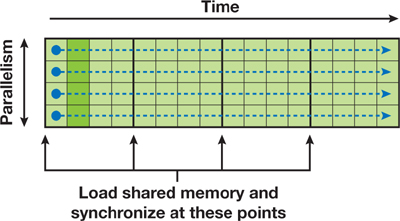
\includegraphics[scale=1.0]{tiles.jpg} 
	\end{center}
	\caption{Tiling and shared memory logic. Image credit: NVIDIA Corporation~\cite{nbody}.}
	\label{fig:1}
	\end{figure}
	
\subsection{Results}
\subsubsection{Warp-based implementation}
Experiments were run for $\texttt{blockSize.x} \in \{256, 512, 1024\}$ with
$\texttt{blockSize.x}= 512$ offering the fastest runtime as shown in listing~\ref{lst:1}.

\begin{lstlisting}[basicstyle=\tiny, frame=single, caption={Task 2: Warp-based force calculation kernel output.}, label={lst:1}]
	Net Force: 0.000000
	Absolute Force: 66480053.035555
	Time: 2.87512449s
	 
	Batch Job Summary Report for Job "nbody_opt" (13789234) on daint
	-----------------------------------------------------------------------------------------------------
	Submit            Eligible               Start                 End    Elapsed  Timelimit 
	------------------- ------------------- ------------------- ------------------- ---------- ---------- 
	2019-05-10T22:29:41 2019-05-10T22:29:41 2019-05-10T22:39:58 2019-05-10T22:40:20   00:00:22   00:02:00 
	-----------------------------------------------------------------------------------------------------
	Username    Account     Partition   NNodes   Energy
	----------  ----------  ----------  ------  --------------
	class04     class01     normal           1          joules
	----------------------------------------------------------
	gpusecs  maxgpusecs        maxmem            summem
	-------  ----------  ------------  ----------------
	3           3     326107136         631242752
	----------------------------------------------------------
	
	\end{lstlisting}

\subsubsection{Shared memory-based implementation}
Experiments were run for $\texttt{blockSize.x} \in \{256, 512, 1024\}$ with
$\texttt{blockSize.x}= 1024$ offering the fastest runtime as shown in listing~\ref{lst:2}.


\begin{lstlisting}[basicstyle=\tiny, frame=single, caption={Task 2: Shared memory-based force calculation kernel output.}, label={lst:2}]
	Net Force: -0.000000
	Absolute Force: 66480053.035555
	Time: 2.30858409s
	 
	Batch Job Summary Report for Job "nbody_opt" (13809329) on daint
	-----------------------------------------------------------------------------------------------------
	Submit            Eligible               Start                 End    Elapsed  Timelimit 
	------------------- ------------------- ------------------- ------------------- ---------- ---------- 
	2019-05-11T16:15:40 2019-05-11T16:15:40 2019-05-11T16:16:16 2019-05-11T16:17:29   00:01:13   00:02:00 
	-----------------------------------------------------------------------------------------------------
	Username    Account     Partition   NNodes   Energy
	----------  ----------  ----------  ------  --------------
	class04     class01     normal           1          joules
	----------------------------------------------------------
	gpusecs  maxgpusecs        maxmem            summem
	-------  ----------  ------------  ----------------
	2           2     326107136         631242752
	----------------------------------------------------------
	\end{lstlisting}

\subsection{Discussion}
Both implementations show a slight aberration from the published naive reference implementation's 
total force value. However, after checking with the responsible lecturer on Piazza this was deemed acceptable.\\
While both kernel implementations reach the 'passing grade with bonus' treshold, only the shared memory-based
kernel reaches the distinction treshold with a runtime of \texttt{2.31s} and thus is submitted as the master result..

\begin{thebibliography}{x}
	% \bibitem{<biblabel>} <citation>
	\bibitem{shuffle}
	  {\scshape Harris, Mark}: {\itshape CUDA Pro Tip: Do the Kepler Shuffle}, NVIDIA Developer Blog, Feb 3, 2014,
	  \url{https://devblogs.nvidia.com/cuda-pro-tip-kepler-shuffle/}, last visited on May 11, 2019.


	\bibitem{nbody}
	  {\scshape Nyland, Lars; Harris, Mark; Prins, Jan}: {\itshape Chapter 31. Fast N-Body Simulation with CUDA}, NVIDIA GPU Gems 3, Aug 12, 2007,
	  \url{https://developer.nvidia.com/gpugems/GPUGems3/gpugems3_ch31.html}, last visited on May 11, 2019.

\end{thebibliography}
\end{document}
